\section{Vanilla SSA (J. Singer)}

\begin{frame}
  \frametitle{Static Single Assignment (SSA)}
\begin{block}{?`SSA?}
  \begin{itemize}
    \item \emph{Assignment}: variable's definition (e.g., \texttt{x} in \texttt{``x=y+1''})
    \item \emph{Single}: only one definition per variable
    \item \emph{Static}: in the program text
  \end{itemize}
\end{block}
\end{frame}

\begin{frame}
\frametitle{Referential transparency}
\begin{block}{Example ($y$ and $z$ are not equal)}
\begin{tabular}{c|c}
opaque (context dependent)& referentially transparent\\
 & SSA form\\ \hline
\begin{minipage}{0.45\textwidth}
\begin{equation*}
\begin{array}{l}
x = 1;\\
y = x + 1;\\
x = 2;\\
z = x + 1;\\
\end{array}
\end{equation*}
\end{minipage} &
\begin{minipage}{0.35\textwidth}
\begin{equation*}
\begin{array}{l}
x_1 = 1;\\
y  = x_1 + 1;\\
x_2 = 2;\\
z  = x_2 + 1;
\end{array}
\end{equation*}
\end{minipage}
\end{tabular}
\end{block}
\pause
\begin{exampleblock}<+->{Referential transparency}
\begin{itemize}
\item value of variable independent of its position
\item may refine our knowledge (e.g., \texttt{``if (x==0)''}) but underlying value of $x$ does not change
\end{itemize}
\end{exampleblock}
\end{frame}

\begin{frame}[fragile,label=inf-semantics]
\frametitle{Informal Semantics}
\vskip1cm
Each variable \texttt{v} is:
\begin{itemize}
  \item used only once as \alert{\texttt{v = \ldots}}
  \hfill (target/definition/left-hand-side)
\item can be many times as \alert{\texttt{\ldots\ = v}}
  \hfill (source/use/right-hand side)

  % \pause
  % \item<+-> but what about when multiple definitions reach a point?
\end{itemize}

% \begin{itemize}
%
% \item phi-function ($\phi$): a pseudo-assignment function ("notational fiction")
% \item multiple definitions of $y$ are renamed as $y_1$ and $y_2$
% \item $\phi$: merge values from different incoming paths\\ at control flow merge points
% \end{itemize}


\pause
\begin{overprint}
  \onslide<+>
  \hskip1cm
   \begin{minipage}{0.4\textwidth}%
\begin{lstlisting}
  $x$ = input();
  if ($x$ == 42) {
    $y$ = 1;
  } else {
    $y$ = $x$ + 2;
  }

  print($y$);
\end{lstlisting}
\end{minipage}
\begin{minipage}{0.5\textwidth}%
\vskip3mm
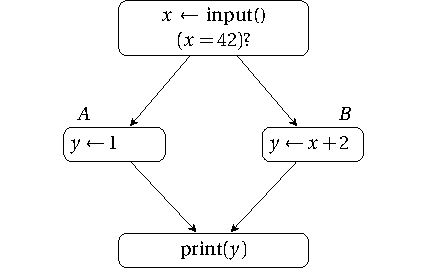
\includegraphics[scale=0.7]{ifthenelse-nonssa.pdf}\goto{CFG}{CFG}
% \hyperlink{CFG}{\beamergotobutton{?`CFG?}}
\end{minipage}

~\vspace{3cm}
%
\onslide<+->
\hskip1cm
\begin{minipage}{0.4\textwidth}
  \begin{center}
% \footnotesize
\begin{lstlisting}
  $x$ = input();
  if ($x$ == 42) {
    $y_1$ = 1;
  } else {
    $y_2$ = $x$ + 2;
  }
  $y_3$ = $\phi$($y_1$,$y_2$);
  print($y_3$);
\end{lstlisting}
  \end{center}
\end{minipage}
\begin{minipage}{0.4\textwidth}
\strut
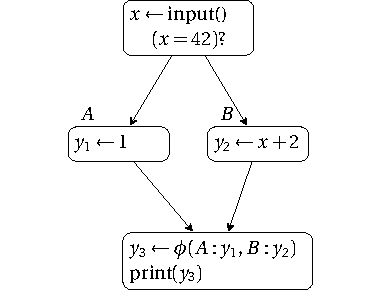
\includegraphics[scale=0.7]{ifthenelse-ssa.pdf}
\end{minipage}
\end{overprint}


\end{frame}

\begin{frame}
\frametitle{Informal Semantics}
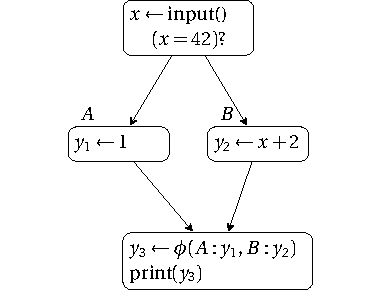
\includegraphics[scale=0.7]{ifthenelse-ssa.pdf}
\begin{minipage}[b]{0.5\textwidth}
  Introduction of $\phi$-functions:
\begin{itemize}
\item to fix the ambiguity; introduces $y_3$ which takes either $y_1$ or $y_2$
\item placed at control-flow merge points i.e., head of basic-blocks that have multiple predecessors
\end{itemize}
\vskip5mm
\end{minipage}
\begin{itemize}
\item $n$ parameters if it has $n$ incoming CFG paths
% \item optionaly can be represented as $a_0=\phi(B_1:a_1, \dots, B_n:a_n)$
\item represented as $a_0=\phi(a_1, \dots, a_n)$
\end{itemize}
\end{frame}


\begin{frame}<handout:0>
  \frametitle{Questions on SSA}
  $\approx$ 5 min to answer the following questions:
  \begin{exampleblock}{}
    Is it possible to have more than one $\phi$-function in a basic block?
  \end{exampleblock}
  \begin{exampleblock}{}
    How can you execute code containing $\phi$-functions on a machine?
  \end{exampleblock}

\end{frame}

\begin{frame}
\frametitle{Informal Semantics}
\begin{itemize}
\item multiple $\phi$-functions executed simultaneously:\\ 
$
\begin{array}{l}
  a=\phi(a',b)\\
  b=\phi(b',a)
\end{array}
$
\item $\phi$-functions not directly executable (IR only: for static analysis)
\item $\phi$-functions removed before assembly code generation\\
  \handr copy instructions insertion
  \pause
\item exists extensions of $\phi$-functions (e.g., $\phi_{\textrm{if}}$, $\gamma$, etc.) that take an additional predicate parameter
\end{itemize}
\end{frame}

\begin{frame}[fragile]
\frametitle{Informal Semantic}
\begin{minipage}[b]{\textwidth}
\begin{itemize}
\item SSA is not Dynamic Single Assignment (DSA or SA)
\item Construction: insert $\phi$-function where multiple reaching defs converge; version variables $x$ and $y$ (integer subscripts); 
\end{itemize}
\end{minipage}

\strut\hfill
\begin{minipage}[t]{0.3\textwidth}
  \begin{lstlisting}
  $x$ = 0;
  $y$ = 0;
  while ($x$<10) {
    $y$ = $y$ + $x$;
    $x$ = $x$ + 1;
  }
  print ($y$);
  \end{lstlisting}
\end{minipage}
\hfill
\begin{minipage}[t]{0.3\textwidth}
\strut
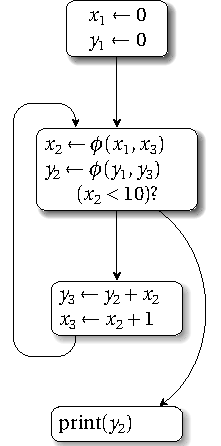
\includegraphics[valign=t,scale=0.65]{while}
\end{minipage}
\hfill\strut
\end{frame}

\begin{frame}
\frametitle{Comparison with Classical Data Flow Analysis}
\begin{itemize}
\item During actual program execution, information flows between variables
\item Static analysis captures this behavior by propagating abstract information along CFG
\item Can be propagated more efficiently using a functional or sparse representation such as SSA
\item Constant propagation: definitions $\equiv$ set of points where information may change; associate information with variable names rather than variables $\times$ program points
%- other data flow problems can be accomodated by inserting additional pseudo-definition functions at appropriate points to induice renaming
\end{itemize}
\end{frame}

\begin{frame}
\frametitle{Comparison with Classical Data Flow Analysis}
\begin{block}{Null pointer analysis}
  \begin{overprint}
    \onslide<+>
    Determine statically if variable can contain null value at run-time.
    \onslide<+->
    \begin{center}
      \footnotesize
      \begin{tabular}[t]{c@{\hskip1cm}c}
      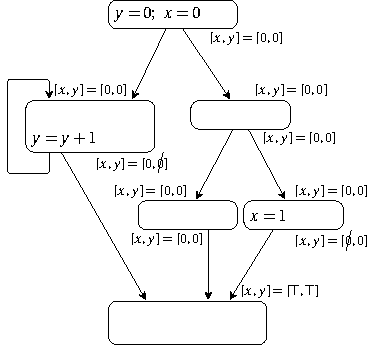
\includegraphics[valign=t,scale=0.7]{zero-1} &
      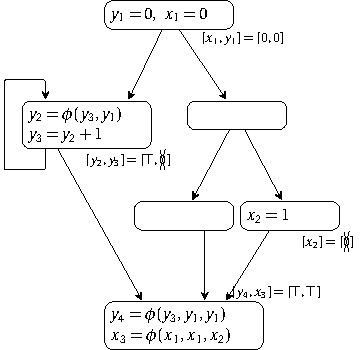
\includegraphics[valign=t,scale=0.7]{zero-2}\\[1ex]
      dense & SSA based
    \end{tabular}
    \end{center}
  \end{overprint}
\end{block}

\uncover<+->{
\begin{itemize}
\item Propagates from defs to uses (via def-use links); avoid program points where information does not change or not relevant
\item Results are more compact
\end{itemize}
}
\end{frame}

\begin{frame}
\frametitle{SSA in Context}
\begin{itemize} 
\item 1980s developments of IRs to encapsulate data dependences to expose direct link between definitions and uses (def-use chains). eg PDG, PD-web... SSA developed at IBM and published late 80s
\item GCC, Open64, HotSpot, Jikes, V8, Mono, LLVM... use SSA
\item more and more popular for JIT compilation on Java byte-code, CLI byte-code, LLVM bitcode...
\item because of favorable properties (simplification and reduced complexity) recently adopted back-end level even register allocation phase
\item also for high-level language impose referential transparency e.g. SISAL; on a per-variable basis final in Java, const or readonly in C\#. Immutability simplifies concurrent programming  
\end{itemize}
\end{frame}

\begin{frame}
\frametitle{Benefits of SSA}
\begin{itemize}
\item Compile time benefit (e.g., sparse data flow analysis)
\item Compiler development benefit (e.g., dead-code in GCC 4.x 40\% of GCC 3.x)
\item Program run-time benefit (simpler to develop more efficient analysis)
\end{itemize}
\begin{center}
\small
\begin{tabular}{p{0.45\textwidth}@{\kern.1\textwidth}p{0.43\textwidth}}
  \hfil Myth\hfil & \hfil Reality \hfil \\[1ex] \hline \\[-2ex]
Greatly increases number of vars & $\approx$10\% expansion\\ [1ex]
Destruction generates many copy ops & not more than original prog. \\ [1ex]
SSA property difficult to maintain & $\equiv$ SSA construction restricted to some variables / code region 
\end{tabular}
\end{center}
\end{frame}


